\chapter{Our contributions}
\label{chap3}

\section{Triangulation adaptive to the local curvature}
\label{sub3.1}

As we explained in the begining of chapeter \ref{sub2.1}, curvature of the surface
is a measure of how much the surface bends.

The triangulation of the surface should be accurate enough, but also memory efficient.
This can be achieved by creating a triangulation which is locally adaptive to the
curvature of the surface. Therefore having smaller triangles in the places where
the surface is curved and having bigger triangles where surface is flatter.

In this section we present our implementation of the triangulation adaptive
to the local curvature.

In the original algorithm, the height of the triangle which is projected
to the surface is set to the constant value $\frac{\sqrt{3}}{2}e$, where $e$ 
is the required length of the side of the triangle. To achieve the adaptivity
of the triangles size, we set the height of the triangle to depend on the curvature in
the given point, as shown in the Figure \ref{img:15}.

\begin{figure}
    \centerline{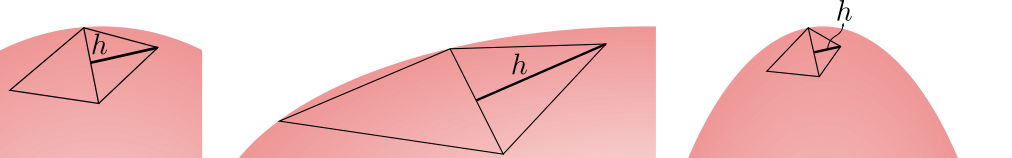
\includegraphics[scale=0.5]{images/img15}}
    \caption[Adaptive height of the new triangle]
    {Adaptive height of the new triangle.}
    %id obrazku, pomocou ktoreho sa budeme na obrazok odvolavat
    \label{img:15}
\end{figure}

To identify the curved areas, we decided to use the maximal curvature. As the minimal
and maximal curvature are both signed, we want to identify the areas depending on 
the absolute value of these curvatures.

We do not allow arbitrary height of the triangle to avoid edge-cases. We decided
to restrict the allowed height to $\frac{1}{4}\frac{\sqrt{3}}{2}e>h>4\frac{\sqrt{3}}{2}e$.
We create a variable $m-$multiplicator, depending on $\kappa_T$ and set the height of
the new triangle to $h=m\frac{\sqrt{3}}{2}e$.

As $\kappa_T$ has values in range $\langle 0, \infty \rangle$.

\begin{definition}
    Let us define triangulation curvature of the surface $S$ in the point $P=S(u, v)$ as
    $\kappa_T(u, v) = max(|\kappa_{min}|, |\kappa_{max}|).$
\end{definition}

NOT FINISHED YET

\section{Triangulation of ADE singularities}
\label{sub3.2}

\subsection*{Analysis of the geometry of ADE singularities}

ADE singularities are simple, isolated surface singularities, which can be
expressed by corresponding implicit equations.

We already know, that $A_{1--}$ singularity is locally represented as a cone.
In this section we discuss geometric structure of other ADE surface singularities.

\begin{definition} (TODO rewrite)
    Let us define branch of ADE singularity as the part of the surface,
    which is connected to the rest only by the singular point.
\end{definition}

\begin{comment}
\begin{definition}
    Let us define triangulation direction of ADE singularity $A$ with radius $r$ as 
    Let us define triangulation direction of ADE singularity $A$ with radius $r$ as 
    a direction $\vec{v}$ for which 
    $$F\bigg(A+t \vec{v} \cap S_{r}(A)\bigg) < 0,$$
    where $F$ is the implicit equation defining the singularity $A$
    and $t,r \in \R^+$.
\end{definition}
As we can see, there are infinitely many axes of each ADE singularity.
\end{comment}

For our needs, we pick one triangulation vector for each branch of
each ADE singularity. This triangulation vector is normalized vector
either in the direction
of rotation symmetry axis or an intersection of reflection symmetry planes
of the corresponding branch. If the branch has only one reflection symmetry
plane, the triangulation vector is picked to lie in the reflection
symmetry plane.

\begin{comment}
Moreover, when placed to the singular point, triangulation vector of a branch 
is in the same half-space as the corresponding branch.
\end{comment}

In the general case, triangulation vectors serve us
as a partial information about the orientation of a singularity with 
respect to its normal form.

\subsubsection*{$A_n$ singularities}

As we can see from the equations 
$F(x,y,z)=x^{n+1}\pm y^2\pm z^2$, $A_{n-+}$
singularities are just rotated $A_{n+-}$ singularities and $A_{n++}$ singularities 
are a single point if $n$ is odd and reflected $A_{n--}$ singularities if $n$ is even. 
We therefore only discuss geometry of $A_{n--}$ and $A_{n+-}$ singularities.

$A_{n--}$ singularities are topologically equivalent to a cone if $n$ is odd, therefore
they have two branches.
If $n$ is even, they are topologically equivalent to a half cone or a plane, therefore
they have a single branch.
As $n$ gets bigger, the tip of the cone gets sharper. As $A_{n--}$ singularities
are rotationally symmetrical, we pick the direction of
axis of symmetry as triangulation vector. For a normal form, the triangulation vectors
are $(1, 0, 0)$ (and $(-1, 0, 0)$ if $n$ is odd).
First four $A_{n--}$ singularities can be seen on the Figure \ref{img:4}.

\begin{figure}
    \centerline{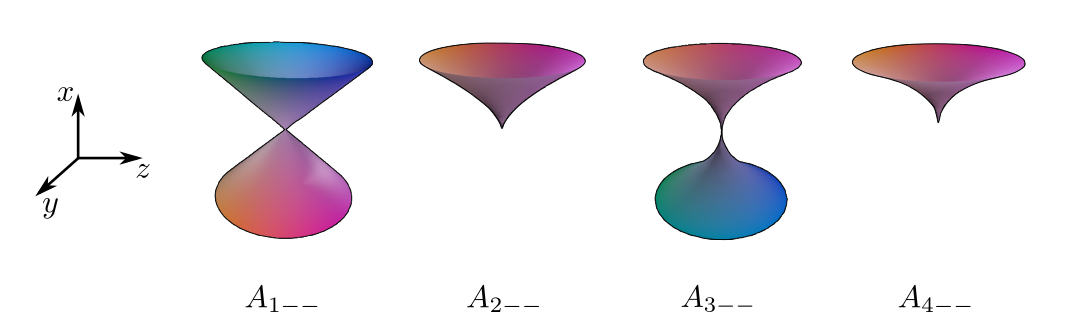
\includegraphics[scale=0.5]{images/img4}}
    \caption[$A_{n--}$ singularities]
    {$A_{n--}$ singularities. \cite{singsurf}}
    %id obrazku, pomocou ktoreho sa budeme na obrazok odvolavat
    \label{img:4}
\end{figure}


$A_{n+-}$ singularities are topologically equivalent to a cone if $n$ is odd, therefore
they have two branches.
In the contrary with the previous singularities, as $n$ gets bigger, the tip
of the cone gets less sharp and flatter. Branches of these singularities have 
reflection symmetry planes $x=0$ and $y=0$, therefore we pick the vectors
$(0, 0, 1)$ and $(0, 0, -1)$ as the triangulation vectors.

If $n$ is even, $A_{n+-}$ singularities are topologically equivalent to a plane
with shape similar to hyperbolic paraboloid, therefore they have a single branch.
First four $A_{n+-}$ singularities can be seen on the Figure \ref{img:5}.
For this case, we pick the vector $(1, 0, 0)$ as a triangulation vector as
these singularities have reflection symmetry planes $y=0$ and $z=0$.

\begin{figure}
    \centerline{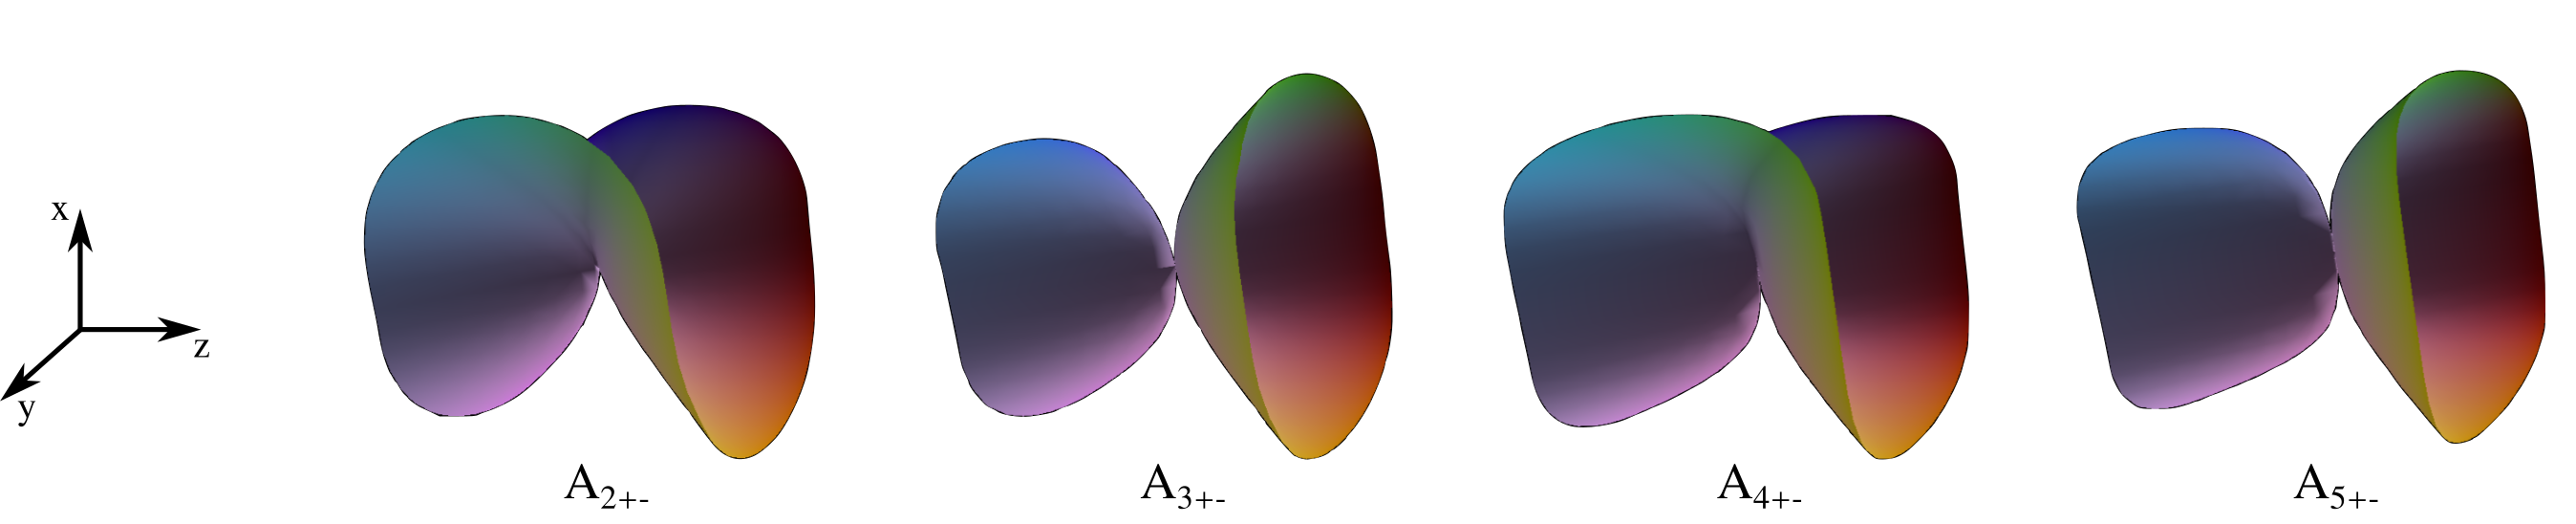
\includegraphics[scale=0.5]{images/img5}}
    \caption[$A_{n+-}$ singularities]
    {$A_{n+-}$ singularities. \cite{singsurf}}
    %id obrazku, pomocou ktoreho sa budeme na obrazok odvolavat
    \label{img:5}
\end{figure}

\subsubsection*{$D_n$ singularities}

Given by equations $F(x,y,z)=yx^2\pm y^{n-1}\pm z^2$, we consider 8 categories.
For given sign combination and parity of n, the singularities are topologically
equivalent, with sharper(or flatter) features around the singularities for increasing
value of $n$ similar to $A_n$ singularities.

We can therefore say that $D_n$ singularities can be classified into 8 categories
locally represented by the following equations:
\begin{itemize}
    \item $D_{4++}$ \hspace{5mm} $yx^2 + y^3 + z^2$
    \item $D_{5++}$ \hspace{5mm} $yx^2 + y^4 + z^2$
    \item $D_{4+-}$ \hspace{5mm} $yx^2 + y^3 - z^2$
    \item $D_{5+-}$ \hspace{5mm} $yx^2 + y^4 - z^2$
    \item $D_{4-+}$ \hspace{5mm} $yx^2 - y^3 + z^2$
    \item $D_{5-+}$ \hspace{5mm} $yx^2 - y^4 + z^2$
    \item $D_{4--}$ \hspace{5mm} $yx^2 - y^3 - z^2$
    \item $D_{5--}$ \hspace{5mm} $yx^2 - y^4 - z^2$.
\end{itemize}

Now we look at some equivalences between these 8 categories.
$D_{4++}$ singularity is reflected $D_{4+-}$ singularity.
$D_{5++}$ singularity is reflected $D_{5--}$ singularity.
$D_{5-+}$ singularity is reflected $D_{5+-}$ singularity.
$D_{4-+}$ singularity is reflected $D_{4--}$ singularity.

We therefore only analyze geometry of $D_{n+-}$ singularities and
$D_{n--}$ singularities.

$D_{n+-}$ singularities are topologically equivalent to a plane when $n$ is
even and to a cone when $n$ is odd. Again, as $n$ gets bigger, the features
around singularities get sharper. Symmetry planes of these singularities
are $x=0$ and $z=0$, therefore we pick $(0, 1, 0)$ (and $(0, -1, 0)$ when $n$ is odd)
as trinauglation vectors. First four $D_{n+-}$ singularities can be seen on
the Figure \ref{img:7}.

\begin{figure}
    \centerline{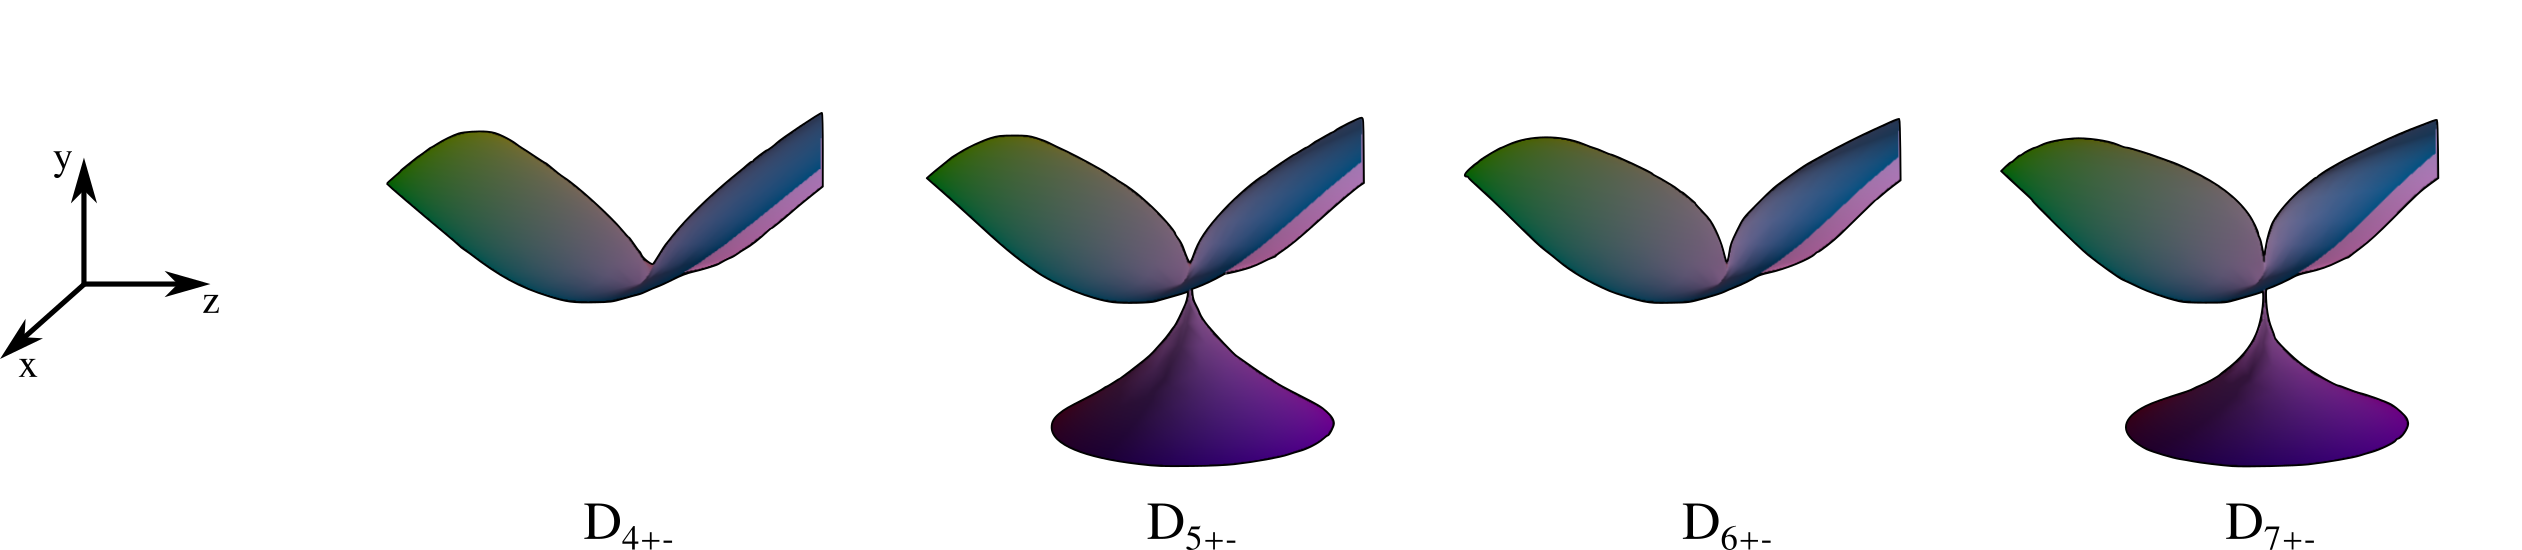
\includegraphics[scale=0.5]{images/img7}}
    \caption[$D_{n+-}$ singularities]
    {$D_{n+-}$ singularities. \cite{singsurf}}
    %id obrazku, pomocou ktoreho sa budeme na obrazok odvolavat
    \label{img:7}
\end{figure}


$D_{n--}$ singularities are topologically equivalent to a cone when $n$ is
odd and to a 3 halfcones connected in the singular point when $n$ is even.
First four $D_{n--}$ singularities can be seen on the Figure \ref{img:8}.

\begin{figure}
    \centerline{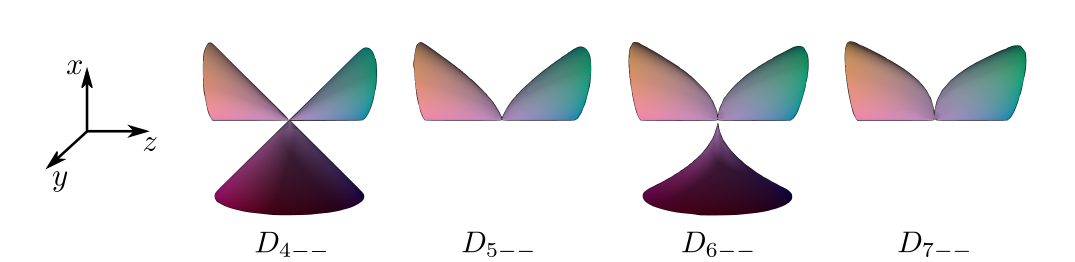
\includegraphics[scale=0.5]{images/img8}}
    \caption[$D_{n--}$ singularities]
    {$D_{n--}$ singularities. \cite{singsurf}}
    %id obrazku, pomocou ktoreho sa budeme na obrazok odvolavat
    \label{img:8}
\end{figure}

Symmetry plane for all branches of these singularities is $z=0$.
the intersection of the surface and plane $z=0$ is displayed on the Figure \ref{img:6}.

\begin{figure}
    \centerline{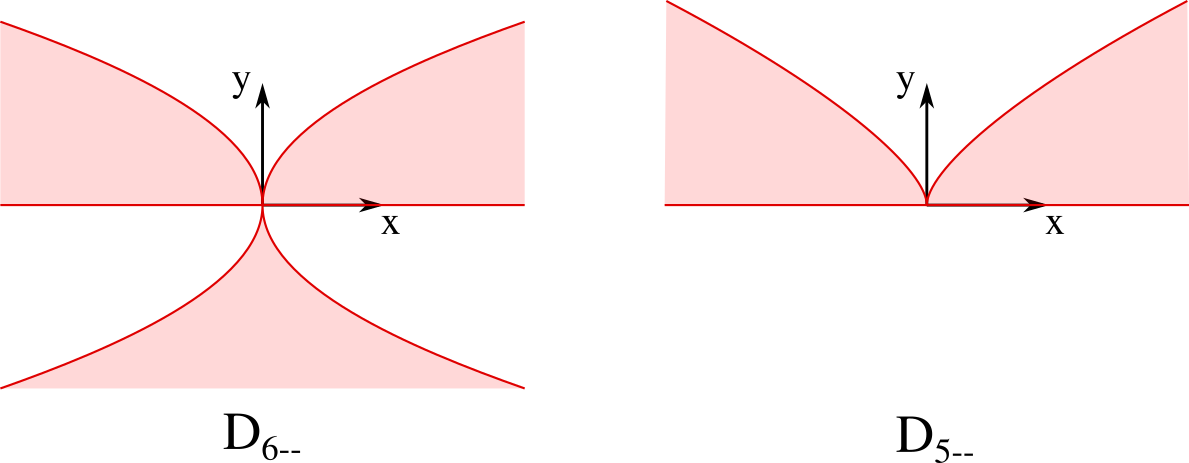
\includegraphics[scale=0.5]{images/img6}}
    \caption[Intersection of $D_{n--}$ singularities with plane $z=0$.]
    {Intersection of $D_{n--}$ singularities with plane $z=0$.}
    %id obrazku, pomocou ktoreho sa budeme na obrazok odvolavat
    \label{img:6}
\end{figure}

For $D_{n--}$ singularity, the intersections of the two branches where
$y \geq 0$ are bounded by curves $y=0$ and $x^2=y^{n-2}$. For given $r$,
we pick the triangulation vectors as $(r, \frac{1}{2}r^{\frac{2}{n-2}}, 0)$
and $(-r, \frac{1}{2}r^{\frac{2}{n-2}}, 0)$. The resulting vectors are
displayed on the Figure \ref{img:9} by blue arrow. Parameter $r$ is changed based
on the length of the edge of triangulation triangle.
displayed on the Figure \ref{img:9} by blue arrow. Parameter $r$ is changed based
on the length of the edge of triangulation triangle.

\begin{figure}
    \centerline{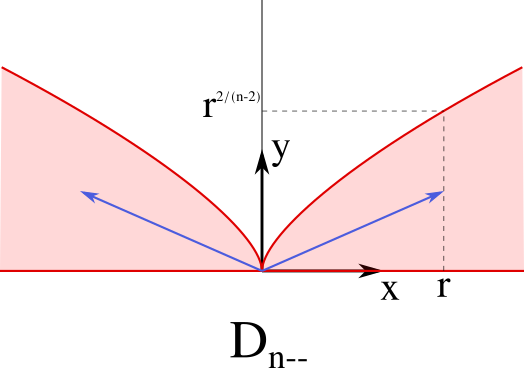
\includegraphics[scale=0.5]{images/img9}}
    \caption[Triangulation vectors for two branches of $D_{n--}$ singularities.]
    {Triangulation vectors for two branches of $D_{n--}$ singularities.}
    %id obrazku, pomocou ktoreho sa budeme na obrazok odvolavat
    \label{img:9}
\end{figure}

The third branch where $y\leq0$ has has another plane of symmetry $x=0$,
therefore triangulation vector for this branch is chosen as $(0, -1, 0)$.

\subsubsection*{$E_6, E_7$ and $E_8$ singularities}

Given by equations $F(x,y,z)=x^3\pm y^4\pm z^2$, $F(x,y,z)=x^3\pm xy^3\pm z^2$
and $F(x,y,z)=x^3\pm y^5\pm z^2$, we can see the following equivalences:
$E_{6++}$ singularity is reflected $E_{6--}$ singularity.
$E_{6+-}$ singularity is reflected $E_{6-+}$ singularity.
$E_{7+-}, E_{7-+}$ and $E_{7--}$ are all reflected $E_{7++}$ singularity.
$E_{8+-}, E_{8-+}$ and $E_{8--}$ are all reflected $E_{8++}$ singularity.

We only analyze geometry of $E_{6++}$, $E_{6+-}$, $E_{7++}$ and $E_{8++}$
singularities. These singularities are displayed on the the Figure \ref{img:12}.


\begin{figure}
    \centerline{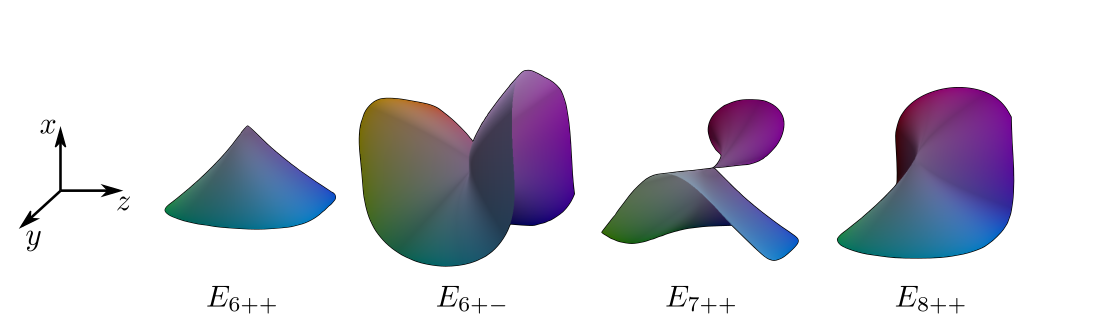
\includegraphics[scale=0.5]{images/img12}}
    \caption[$E_n$ singularities.]
    {$E_n$ singularities. \cite{singsurf}}
    %id obrazku, pomocou ktoreho sa budeme na obrazok odvolavat
    \label{img:12}
\end{figure}
Both $E_{6++}$ and $E_{6+-}$ are topologically equivalent to a plane, thus
they each have only one branch. The planes of symmetry of both of these 
branches are $y=0$ and $z=0$, therefore we pick $(-1, 0, 0)$ as the
triangulation vector.

$E_{7++}$ singularity is topologically equivalent to a cone, therefore it has
two branches. The plane of symmetry of this singularity is $z=0$.

$E_{8++}$ singularity is also topologically equivalent to a plane, therefore
it has only one branch. This branch has only one plane of symmetry $z=0$.

We again look at the intersection of the surfaces with the plane of 
symmetry, this is displayed on the Figure \ref{img:10}.

\begin{figure}
    \centerline{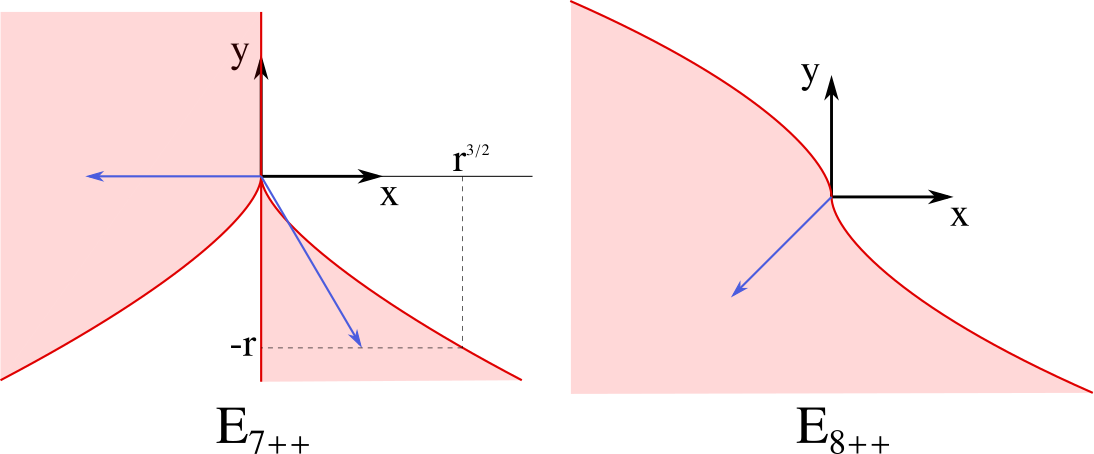
\includegraphics[scale=0.5]{images/img10}}
    \caption[Intersection of $E_{7++}$ and $E_{8++}$ singularities with 
    plane $z=0$.]
    {Intersection of $E_{7++}$ and $E_{8++}$ singularities with 
    plane $z=0$.}
    %id obrazku, pomocou ktoreho sa budeme na obrazok odvolavat
    \label{img:10}
\end{figure}

For $E_{7++}$ singularity, we pick $(-1, 0, 0)$ and 
$(\frac{1}{2}r^{\frac{3}{2}}, -r, 0)$ as triangulation vectors.
For $E_{8++}$ singularity, we pick $(-1, -1, 0)$ as a triangulation vector.
These vectors are displayed on the Figure \ref{img:10} as blue arrows.

\subsection*{Analytical calculation of local triangulation of some ADE singularities}
For given edge size $e$, we want to calculate the local triangulation of ADE
singularities, such that edges on the border of the local triangulation
have length $e$.
\subsubsection*{$A_{n--}$ singularities}
For $A_{n--}$ singularities, we create a disc of six isosceles triangles
with vertex in the singular point. The bases of these triangles create regular
hexagon in the plane $P$ parallel to the plane $x=0$, as showed on the Figure
\ref{img:11}.
\begin{figure}
    \centerline{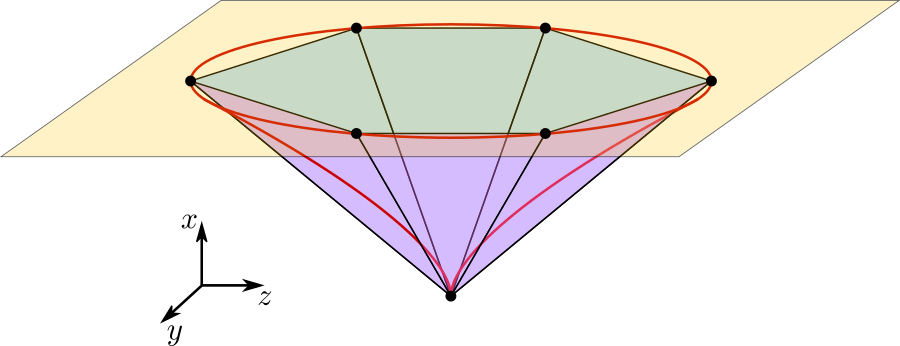
\includegraphics[scale=0.5]{images/img11}}
    \caption[Triangulation of $A_{n--}$ singularity.]
    {Triangulation of $A_{n--}$ singularity.}
    %id obrazku, pomocou ktoreho sa budeme na obrazok odvolavat
    \label{img:11}
\end{figure}
Given by equation $x^{n+1}-y^2-z^2=0$, we find the distance of the 
plane $P$ from the plane $x=0$ for the given length $e$ of the sides of
the hexagon.

Let $e$ be the length of the side of the hexagon, then the circumscribed
circle has radius $e$. This circle is identical with the intersection of
the surface and the plane $x=h$. The equation of the intersecting circle
is $y^2+z^2=h^{n+1}$ therefore, the radius can be also expressed as 
$r=h^{\frac{n+1}{2}}$, which emerges $h=e^{\frac{2}{n+1}}$. Knowing the
distance of the plane, one can easily calculate the length of the arms of
the triangles using Pythagorean theorem: 
$$a^2=h^2+e^2 \implies a = \sqrt{e^{\frac{4}{n+1}} + e^2}$$

\subsubsection*{$D_n$ singualrities}
Some $D_n$ singularities have branches with elliptical intersection with 
a plane parallel to the plane $y=0$. As ellipses have two axes of symmetry,
we create eight triangles with apex in the singular point for these branches.
The other points of the triangles lie on the ellipse and they have the same length
of the base.

Let us have an ellipse $E$ with semi-major axis $a$, semi-minor axis $b$ 
and the center in the point $(0, 0)$.

$$E: \frac{x^2}{a^2} + \frac{y^2}{b^2} = 1$$
\begin{figure}
    \centerline{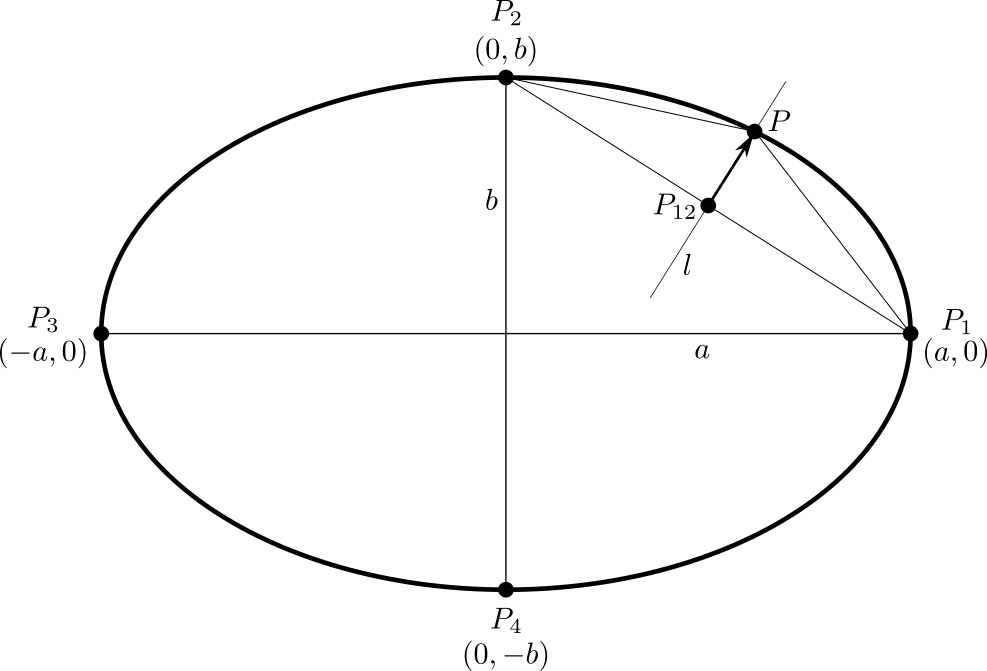
\includegraphics[scale=0.5]{images/img13}}
    \caption[Equidistant points on ellipse.]
    {Equidistant points on ellipse.}
    %id obrazku, pomocou ktoreho sa budeme na obrazok odvolavat
    \label{img:13}
\end{figure}
As displayed on the Figure \ref{img:13}, we pick the leftmost, the rightmost, the top
and the bottom points. As shown on the figure \ref{img:13}, the coordinates of these 
points are $P_1 = (a, 0)$, $P_2 = (0, b)$, $P_3=(-a, 0)$, $P_4 = (0, -b)$.
Then we can calculate the point $P$ on ellipse equidistant
from points $P_1$ and $P_2$. We calculate this point by taking the point $P_{12}$ 
in the middle of a line segment $P_1P_2$. 

$$P_{12} = \frac{1}{2}(a, b)$$

Then, the point $P$ is lying on the
intersection of the ellipse and a line $l$ passing through the point $P_{12}$, perpendicular to the
line segment $P_1P_2$.

$$l: \frac{1}{2}(a,b) + \frac{t}{2}(b,a), \hspace{3mm} t \in \R$$

Given the ellipse with semi-major axis $a$, 
semi-minor axis $b$ and the center in the point $(0, 0)$, the point $P$ can be 
calculated as follows:

$$P \in l \cap E \implies 
\frac{(a+tb)^2}{4a^2} + \frac{(b+ta)^2}{4b^2} = 1$$
$$t=\frac{ab(\sqrt{3a^4+2a^2b^2+3b^4}-a^2-b^2)}{a^4+b^4},$$

therefore 
$$P=\frac{1}{2}(a,b) + \frac{ab(\sqrt{3a^4+2a^2b^2+3b^4}-a^2-b^2)}{2(a^4+b^4)}(b,a).$$

TODO binary search for height

Given edge length $e$, we are not able to calculate the height in which the distance
between points $P1$ and $P$ is $e$. The visualization showing this is on the Figure \ref{img:17}.

\begin{figure}
    \centerline{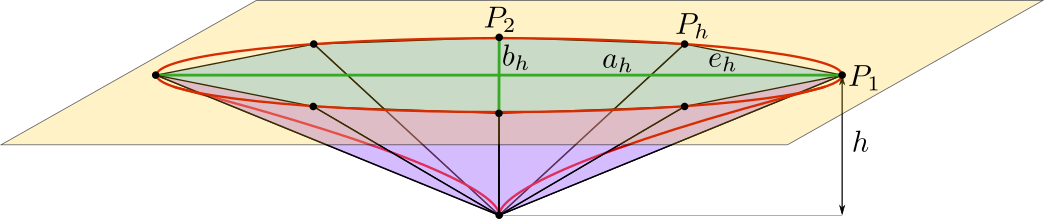
\includegraphics[scale=0.5]{images/img17}}
    \caption[Calculating the point $P_h$]
    {Calculating the point $P_h$ -- point on the ellipse equidistant from $P_1$ and $P_2$.}
    %id obrazku, pomocou ktoreho sa budeme na obrazok odvolavat
    \label{img:17}
\end{figure}

We use binary search to find such height.
Given the height and the singularity class, we can calculate the semi-major axis
and semi-minor axis as 

$$D_{n+-} \hspace{3mm} :\hspace{3mm}  -hx^2+h^{n-1}-z^2 = 0 \hspace{5mm} h>0$$
$$x^2 + \frac{z^2}{h} = h^{n-2}$$
$$\frac{x^2}{h^{n-2}} + \frac{z^2}{h^{n-1}} = 1 \implies a_h=max(h^\frac{n-2}{2}, h^\frac{n-1}{2}) \land b_h=min(h^\frac{n-2}{2}, h^\frac{n-1}{2}).$$

As we can see, we get the same ellipse for $D_{n--}$ singularities:

$$D_{n--} \hspace{3mm} :\hspace{3mm}  -hx^2-h^{n-1}-z^2 = 0 \hspace{5mm} h>0$$
$$2|n \land x^2 + \frac{z^2}{h} = -h^{n-2} \implies x^2 + \frac{z^2}{h} = h^{n-2}.$$
Then 
$$P_h=\frac{1}{2}(h^\frac{n-2}{2},h^\frac{n-1}{2}) + \frac{h^\frac{2n-3}{2}(\sqrt{3h^{2n-4}+2h^{2n-3}+3h^{2n-2}}-h^{n-2}-h^{n-1})}{2(h^{2n-4}+h^{2n-2})}(h^\frac{n-1}{2},h^\frac{n-2}{2})$$
$$P_h=\frac{1}{2}(h^\frac{n-2}{2},h^\frac{n-1}{2}) + \frac{h^\frac{1}{2}(\sqrt{3+2h+3h^2}-1-h)}{2(1+h^2)}(h^\frac{n-1}{2},h^\frac{n-2}{2})$$
and we can calculate $e_h=||P_h-P_1||$.

As $e \leq a_h$, we can start the binary search on the interval
$\langle 0, a^\frac{2}{n-2}\rangle$ or $\langle 0, a^\frac{2}{n-1}\rangle$
and finish, when required precision is reached.

TODO want to try to prove that $||P_h-P_1||$ is monotone in h.

\subsection*{Numerical calculation of local triangulation of ADE singularities}

For other types of ADE singularities, the exact analytical calculations become more
complicated. In this section we present an approach for triangulation of all types
of ADE singularities using numerical algorithms such as binary search.

We begin by dividing ADE singularities into three categories.
\begin{enumerate}
    \item Singularities topologically equivalent to a plane:
    \begin{itemize}
        \item $A_{n--}$, where $2|n$,
        \item $A_{n+-}$, where $2|n$,
        \item $D_{n+-}$, where $2|n$,
        \item $E_{6++}$, 
        \item $E_{6+-}$,
        \item $E_{8++}$.
    \end{itemize}
    \item Singularities topologically equivalent to a cone except $E_{7++}$:
    \begin{itemize}
        \item $A_{n--}$, where $2 \nmid n$,
        \item $A_{n+-}$, where $2 \nmid n$,
        \item $D_{n+-}$, where $2 \nmid n$,
        \item $D_{n--}$, where $2 \nmid n$
    \end{itemize}
    \item Other singularities:
    \begin{itemize}
        \item $D_{n--}$, where $2|n$,
        \item $E_{7++}$.
    \end{itemize}
\end{enumerate}

We propose a general solution for first and second categories and we treat the
singularities in the third category as a special cases.

\subsubsection*{Singularities topologically equivalent to a plane}
\subsubsection*{Singularities topologically equivalent to a cone except $E_{7++}$}
\subsubsection*{Other singularities - special cases}

\subsection*{Triangulation of a plane with multiple $A_{n--}$ singularities}
In this section, we present an approach for creating an implicit equation of a
surface which consists of a plane and arbitrary many $A_{n--}$ singularities
$C^1$ smoothly connected to this plane. 
\subsubsection*{Input and output}
In this section, the following data are provided on the input:
\begin{enumerate}
    \item the number of singularities - $m$,
    \item $m$ discrete points on a plane - $(x_1, y_1), ..., (x_m, y_m)$,
    \item $m$ degrees of the singularities - $n_1, ..., n_m$,
    \item $m$ heights at which each singularity is connected - $h_1, ..., h_m$.
\end{enumerate}
The visualisation of desired output function can be seen on the Figure \ref{img:22}. 
On this figure, the singularity is displayed by green color, the red color is used to
display the function which connects the singularity to a plane - the bump function.
\begin{figure}
    \centerline{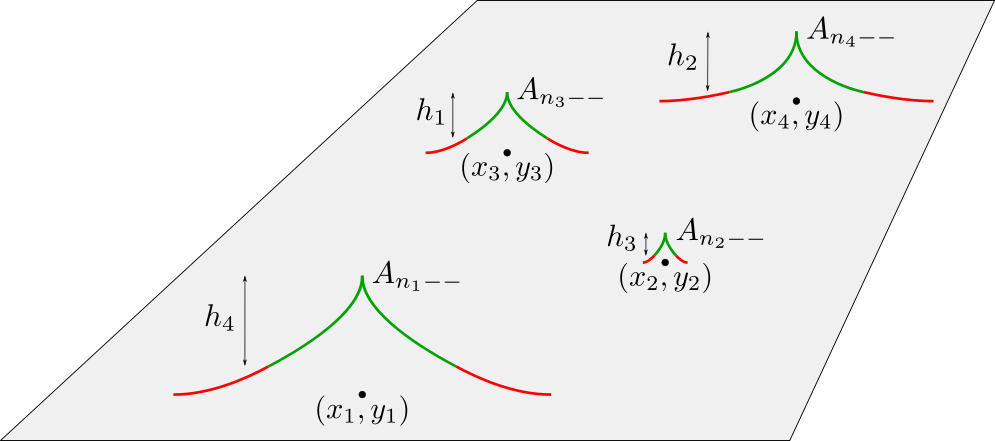
\includegraphics[scale=0.5]{images/img22}}
    \caption[Plane with singularities.]
    {Plane with singularities.}
    %id obrazku, pomocou ktoreho sa budeme na obrazok odvolavat
    \label{img:22}
\end{figure}
There are some limitations on the input data. As we do not want the singularities 
or the bump functions to intsect, we require that each pair of input points is
distanced $d_{ij}$ from each other. We specify the value of $d_{ij}$ in the section TODO.
\subsubsection*{Bump function}
\begin{definition}
The support $supp(f)$ of a function $f: \R^n \to \R$ is a set of points where $f$ is not
zero: $$supp(f) = \{ x\in \R^n : f(x)\neq 0 \}.$$
The closed support of the function $f$ is defined as a closure of $supp(f)$.
\end{definition}
Bump function if a function $f:\R^n \to \R$ which is smooth ($C^\infty$) and
compactly supported (the closed support of the function $f$ is a compact subset
of $\R^n$).

The most common example of such bump function is the function 
$$f(x)= \left\{
    \begin{array}{ll}
        e^{-\frac{1}{1-x^2}}, & x \in (-1, 1) \\
          0, & otherwise,\\
    \end{array} 
    \right. $$
which is both $C^\infty$ and compactly supported.

The bump function can be used to smoothly connect a curve to a line or a surface to a
plane in higher dimension. If we only need to connect a curve and a line $C^n$ smoothly, 
we only need a bump function which connects $C^n$ smoothly to a line.

In our work, we connect two surfaces with $C^1$ continuity and for this purpose
we use the function
$$f(x)= \left\{
    \begin{array}{ll}
        -q \cdot cos(k \cdot x)-q, & x \in (-\frac{\pi}{k}, \frac{\pi}{k}) \\
        0, & otherwise,\\
    \end{array} 
    \right. $$
rotated about $z$-axis.
The result of the rotation is the following function:
$$f(x, y) = \left\{
    \begin{array}{ll}
        -q \cdot cos(k \cdot (x^2+y^2))-q, & x^2+y^2<=(\frac{\pi}{k})^2 \\
        0, & otherwise.\\
    \end{array} 
    \right. $$
Both of these functions can be seen on the Figure \ref{img:21}.
\begin{figure}
    \centerline{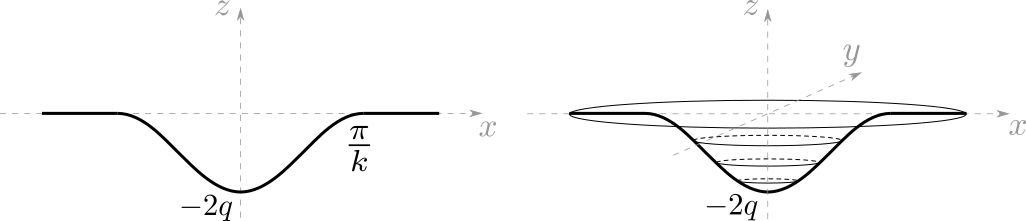
\includegraphics[scale=0.5]{images/img21}}
    \caption[$C^1$ cosine bump function.]
    {$C^1$ cosine bump function.}
    %id obrazku, pomocou ktoreho sa budeme na obrazok odvolavat
    \label{img:21}
\end{figure}

\subsubsection*{Implicit equation of the cosine bump function}
To construct the implicit equation of the cosine bump function, we use CSG
- constructive solid geometry, which is described in the section \ref{sub2.6}.

First, we cut out the part of the rotated cosine, where
$x^2+y^2<(\frac{\pi}{k})^2$ using cylinder and intersection operation. Next,
we use a plane and the union operation to \textit{glue} the bump to the plane.
The described process is displayed on the Figure \ref{img:24} in the form of CSG tree.
\begin{figure}
    \centerline{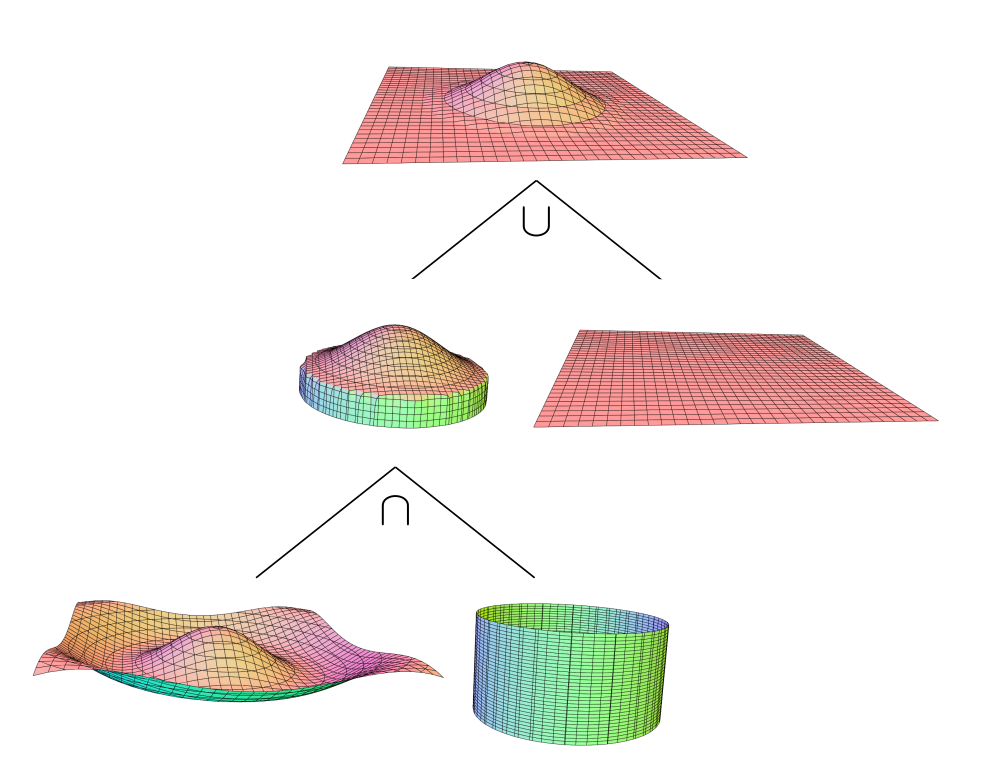
\includegraphics[scale=0.5]{images/img24}}
    \caption[Construction of the cosine bump function using CSG]
    {Construction of the cosine bump function using CSG.}
    %id obrazku, pomocou ktoreho sa budeme na obrazok odvolavat
    \label{img:24}
\end{figure}
We use the following equations of the surfaces to model the cosine bump function:

\begin{table}[]
    \centering
    \begin{tabular}{|c|c|}
        \hline\hline
    Funcion name            & Implicit equation                                        \\ \hline\hline
    Rotated cosine function & $x+q \cdot cos(k \cdot \sqrt{(y-p_y)^2+(z-p_z)^2})+q=0$  \\ \hline
    Cylinder                & $(y-p_y)^2+(z-p_z)^2-(\frac{\pi}{k})^2=0$                \\ \hline
    Plane                   & x=0                                                      \\ \hline\hline
    \end{tabular}
    \caption[Implicit equations for bump function modeling]
    {Implicit equations for bump function modeling.}
    \label{tab:1}
    \end{table}

Parameters $q$ and $k$ allow us to change the amplitude and the frequency of
the cosine function, parameters $p_y$ and $p_z$ are used to move the bump function
to the given point $(p_y, p_z)$.

\subsubsection*{Attaching singularities to the plane using the cosine bump function}

Given the type of the singularity - $n$ and given height - $h$, we calculate the
constants of the cosine bump function to connect $C^1$ smoothly to the given
singularity.

The singularity given by the implicit equation $x^{n+1}-y^2-z^2$ intersected with 
the plane $x=h$ produces a circle with the radius $r=\sqrt{h^{n+1}}$.
The cosine bump function is scaled using $q$ and $k$ to smoothly connect the
singularity in the middle of the cosine bump function. This approach is displayed
on the Figure \ref{img:25}. 

\begin{figure}
    \centerline{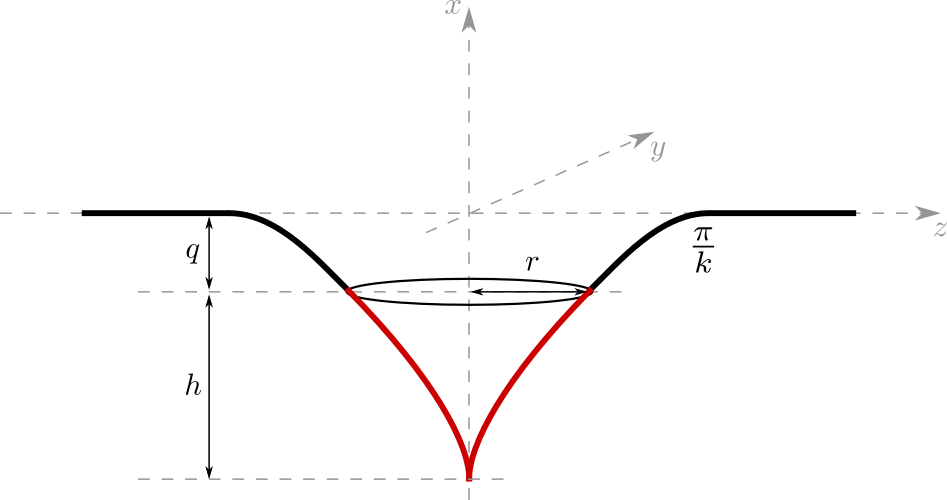
\includegraphics[scale=0.5]{images/img25}}
    \caption[Attaching the singularity to a plane using the cosine bump function]
    {Attaching the singularity to a plane using the cosine bump function.}
    %id obrazku, pomocou ktoreho sa budeme na obrazok odvolavat
    \label{img:25}
\end{figure}

As the singularity is attached in the middle of the
bump function, we get the equality $r=\frac{\pi}{2k}$ and therefore
$\sqrt{h^{n+1}}=\frac{\pi}{2k} \implies k=\pi/(2\sqrt{h^{n+1}})$.
The parameter $q$ is calculated from $C^1$ continuity requirement. We require the
gradients to be linearly dependent in the points of connection. Due to the rotation
symmetry, we check it only for the intersection with the plane $z=0$
for the point $(-q, \frac{\pi}{2k})$.
$$F=(x+h+q)^{n+1}-y^2 \implies \nabla F = \left[(n+1)(x+h+q)^n, -2y\right]$$
$$\nabla F \left(-q, \frac{\pi}{2k}\right) = \left[(n+1) h^n, -\frac{\pi}{k}\right]$$
$$G=x+q \cdot cos(k y)+q \implies \nabla G = \left[1, -qk \cdot sin(k y)\right]$$
$$\nabla G \left(-q, \frac{\pi}{2k}\right) = \left[1, -qk \right]$$

Requiring $\nabla F (-q, \frac{\pi}{2k}) = s \cdot \nabla G (-q, \frac{\pi}{2k})$
and knowing $k=\pi/(2\sqrt{h^{n+1}})$, we get $s=(n+1)h^n$ and therefore $q=4h/(\pi(n+1))$.

After calculating the parameters $q$ and $k$ of the cosine bump function, 
we proceed to connect the singularity to the bump function.
We use intersection with the plane $x=-q$ to get the sections of the singularity
and the section of the bump function and lastly, we use union of these two 
surfaces. The described process is displayed on the Figure \ref{img:26}.
Curious reader can find the detailed calculation of the implicit equation in
the appendix \ref{appA}.

\begin{figure}
    \centerline{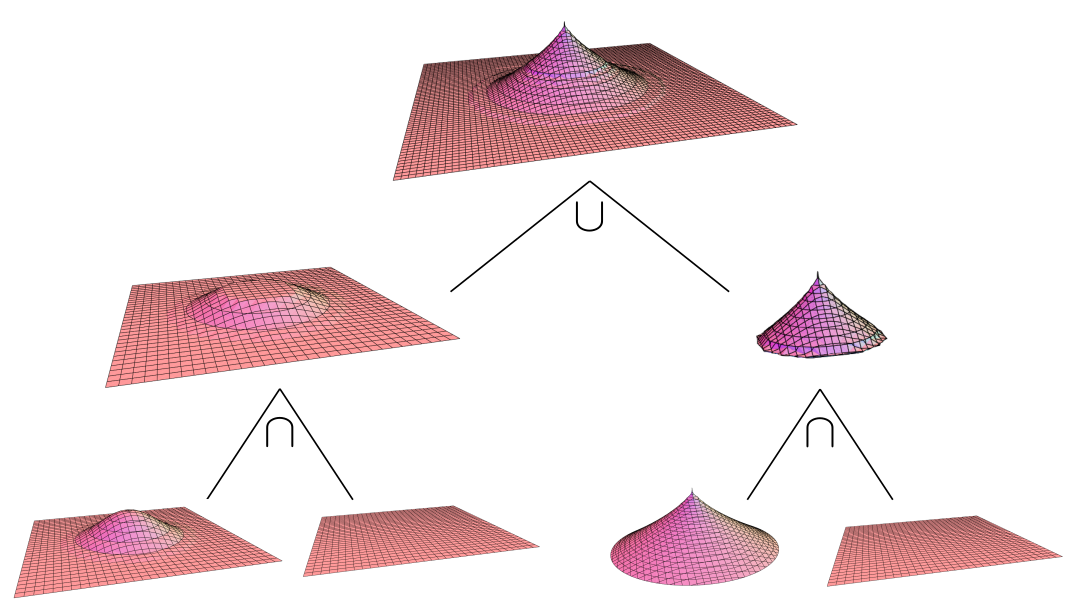
\includegraphics[scale=0.5]{images/img26}}
    \caption[Attaching the singularity to a plane using CSG]
    {Attaching the singularity to a plane using CSG.}
    %id obrazku, pomocou ktoreho sa budeme na obrazok odvolavat
    \label{img:26}
\end{figure}

To connect multiple singularities to the same plane, we construct the implicit
equation for each of these singularities and then use the union operation to
create a surface with multiple singularities. This procedure is displayed on
the Figure \ref{img:28}.

\begin{figure}
    \centerline{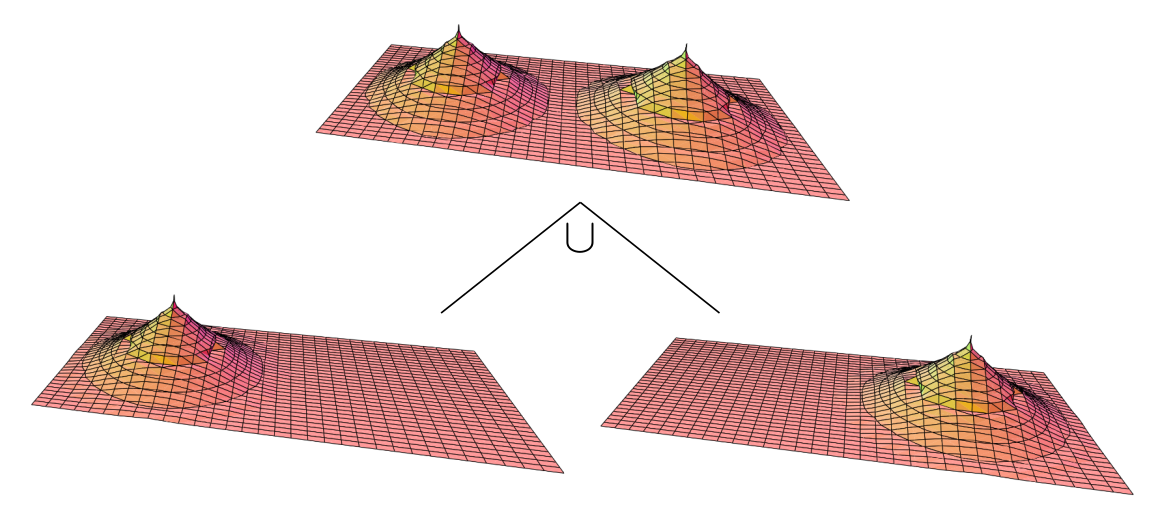
\includegraphics[scale=0.5]{images/img28}}
    \caption[Plane with multiple attached singularities]
    {Plane with multiple attached singularities.}
    %id obrazku, pomocou ktoreho sa budeme na obrazok odvolavat
    \label{img:28}
\end{figure}

\subsubsection*{Limitations on the input data}
As we already mentioned, we require that each pair of input points is
distanced $d_{ij}$ from each other. As the radius of the closed support
of the cosine bump function is $r=\frac{\pi}{k}=2\sqrt{h^{n+1}}$, the 
distance between two input points $p_j, p_j$ must be at least
$d_{ij} = 2\sqrt{h_i^{n_i+1}}+2\sqrt{h_j^{n_j+1}}$. This way, both singularities
and the corresponding bump functions do not intersect. 

\subsubsection*{Visualization of results of the triangulated surfaces}

\section{Triangulation of non-isolated singularities}
\label{sub3.3}
